\section{Introduction}
\label{sec:intro}

Repository-level software engineering relies on agents navigating complex dependencies and reasoning about high-level architectural intent~\citep{wang2025improving, zhao2025towards}. However, as illustrated in Figure~\ref{fig:intention}, existing approaches suffer from a reasoning gap due to fragmented representations: \textbf{API Documentation} focuses on semantic intent~\citep{luo2024repoagent, chen2025llms} but lacks global navigability, forcing models to infer architectural connectivity~\citep{chen2025towards, jain2025mitigating}. Conversely, \textbf{Dependency Graph} captures structural logic~\citep{ouyang2024repograph, ma2024understand} but provide limited semantic information~\citep{borowski2024semantic, cheng2024semantic}, leaving agents to follow execution paths without reflecting the underlying rationale~\citep{jiang2025cosil}. Furthermore, maintaining consistency incurs prohibitive overhead: documentation is prone to semantic drift~\citep{tan2024detecting}, while static graphs capture syntactic updates but often overlook logical implications~\citep{groninger2025changeguard}.


\begin{figure}[ht] 
\centering
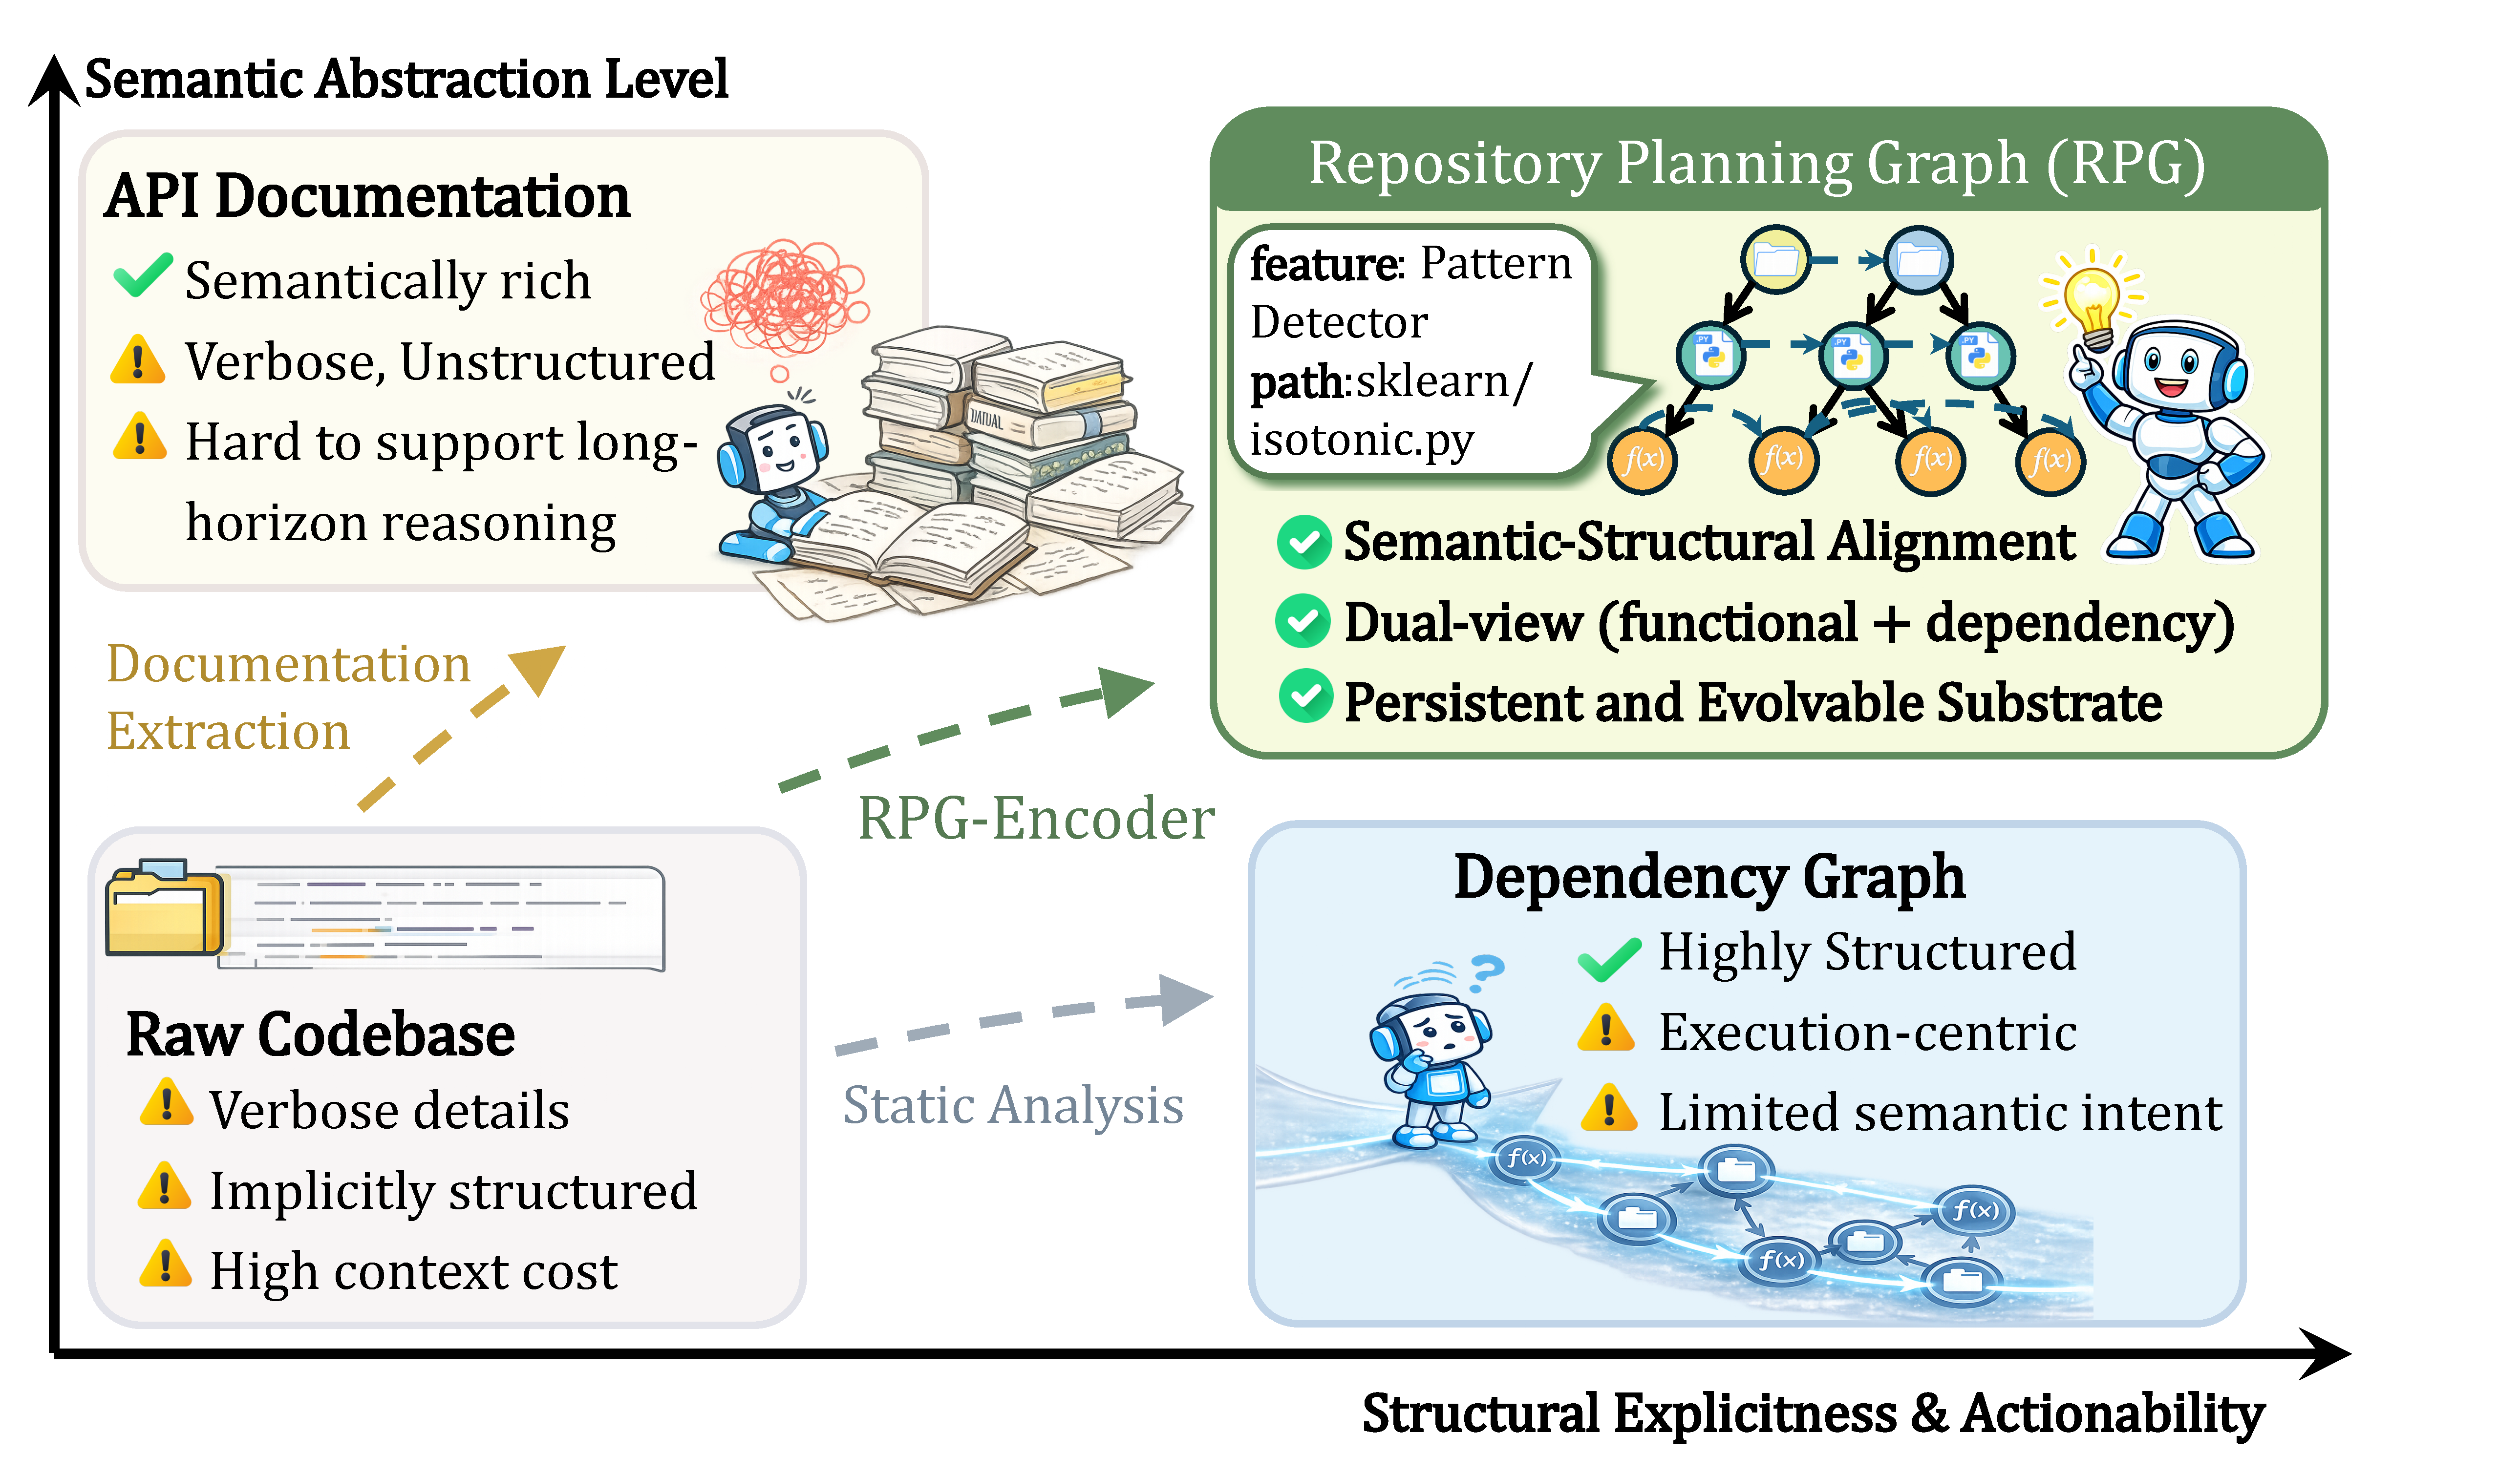
\includegraphics[width=\linewidth]{figs/encoder_intention.pdf}
\caption{Comparison of code representations regarding semantic abstraction and structural explicitness. Unlike approaches limited to a single dimension, RPG achieves dual-view alignment, combining semantic richness with structural actionability.} 
\label{fig:intention}
\vspace*{-5pt} 
\end{figure}

We observe that this reasoning disconnect is not merely a failure of individual tools, but a systemic consequence of treating repository understanding as an isolated, unidirectional task. Fundamentally, this occurs because current approaches ignore the inherent symmetry of software engineering.
We argue that repository comprehension and generation constitute inverse pathways within a unified reasoning cycle: generation expands sparse intent into detailed code, whereas comprehension must compress noisy implementation back into high-level intent. Consequently, bridging this gap requires a \textbf{unified Intermediate Representation} that fuses the semantic density of documentation with the topological rigor of dependency graphs. The Repository Planning Graph (RPG)~\citep{luo2025rpg_zerorepo} emerges as a suitable representation for this unification. Having served as a generative blueprint for intent-to-code, it possesses the dual-view structure needed for the inverse code-to-intent journey. This motivates our fundamental inquiry: \textit{Can the RPG be generalized to serve as a unified, high-fidelity representation for existing repositories, thereby closing the loop?}


To realize this vision, we propose \ours{}, a framework that transforms the RPG from a static generative blueprint into a dynamic, bidirectional representation. We implement this through three cohesive mechanisms:
(1) \textbf{Encoding:} We introduce a semantic lifting protocol that projects code into the RPG. Nodes combine functional descriptions with code metadata, while edges encode hierarchy and static dependencies, yielding an interpretable and verifiable representation.
(2) \textbf{Evolution:} We design an incremental mechanism that parses commit diffs to update the RPG. This keeps semantics synchronized with implementation without re-generation.
(3) \textbf{Operation:} We establish the RPG as a unified interface for structure-aware reasoning. It serves as a topological map, enabling traversal between high-level intent and low-level execution logic.


To evaluate the extracted RPG, we conduct a dual-task evaluation on two critical dimensions: navigational utility and representational fidelity. (1) In \textbf{Repository Understanding}, \ours{} with Claude-4.5-Sonnet~\citep{anthropic_claude_sonnet_4_5} demonstrates superior function-level performance, achieving 93.7\% Acc@5 on SWE-bench Verified~\citep{jimenez2023swe} and exceeding the best baseline by over 10\% on SWE-bench Live Lite~\citep{zhang2025swe}. This confirms that coupling semantic features with topology significantly strengthens fine-grained localization. (2) In \textbf{Repository Reconstruction}, \ours{} outperforms API documentation by providing an explicitly ordered blueprint. Guided by topological constraints, \ours{} reconstructs repositories with 98.5\% coverage (+24.3\% over baselines) and 86.0\% pass rate on RepoCraft~\citep{luo2025rpg_zerorepo}. In contrast, documentation lacks structural guidance and recovers only $\sim 17\%$ of the original code volume, proving that RPG serves as a structured representation that effectively preserves complete repository semantics. Analysis confirms that semantic features are essential for effective exploration, and our incremental strategy reduces maintenance costs by 95.7\% without incurring semantic drift.

Our contributions are summarized as follows:
\begin{itemize}
    \item We generalize the Repository Planning Graph (RPG) into a unified representation that closes the loop between comprehension and generation, theoretically grounding repository reasoning as a unified reasoning cycle where semantic intent and structural dependencies are bidirectionally linked. 

    \item We introduce \ours{}, a framework that implements a semantic lifting protocol to recover high-level intent from code and supports sustainable evolution via differential updates, decoupling maintenance costs from repository scale.

    \item We validate \ours{} on dual tasks: establishing SOTA performance in repository understanding to demonstrate superior navigational utility, and achieving 98.5\% coverage in repository reconstruction to verify its high-fidelity representational capacity.
\end{itemize}